% !TeX spellcheck = en_US

%
% This is a borrowed LaTeX template file for lecture notes for CS267,
% Applications of Parallel Computing, UCBerkeley EECS Department.
% Now being used for CMU's 10725 Fall 2012 Optimization course
% taught by Geoff Gordon and Ryan Tibshirani.  When preparing 
% LaTeX notes for this class, please use this template.
%
% To familiarize yourself with this template, the body contains
% some examples of its use.  Look them over.  Then you can
% run LaTeX on this file.  After you have LaTeXed this file then
% you can look over the result either by printing it out with
% dvips or using xdvi. "pdflatex template.tex" should also work.
%

\documentclass[twoside]{article}
\setlength{\oddsidemargin}{0.25 in}
\setlength{\evensidemargin}{-0.25 in}
\setlength{\topmargin}{-0.6 in}
\setlength{\textwidth}{6.5 in}
\setlength{\textheight}{8.5 in}
\setlength{\headsep}{0.75 in}
\setlength{\parindent}{0 in}
\setlength{\parskip}{0.1 in}

%
% ADD PACKAGES here:
%
\usepackage{graphicx}
\usepackage{amsmath,amsfonts,graphicx}
\usepackage{algorithm}
\usepackage{algorithmic}
\usepackage{lipsum}
 \usepackage[margin=1in]{geometry} 
\usepackage{amsthm,amssymb}
\usepackage{bm}
\usepackage{enumerate}
\usepackage{booktabs}
%\renewcommand{\familydefault}{pag}
%\renewcommand{\familydefault}{pbk}
% https://en.wikibooks.org/wiki/LaTeX/Fonts

%
% The following commands set up the lecnum (lecture number)
% counter and make various numbering schemes work relative
% to the lecture number.
%
\newcounter{lecnum}
\renewcommand{\thepage}{\thelecnum-\arabic{page}}
\renewcommand{\thesection}{\thelecnum.\arabic{section}}
\renewcommand{\theequation}{\thelecnum.\arabic{equation}}
\renewcommand{\thefigure}{\thelecnum.\arabic{figure}}
\renewcommand{\thetable}{\thelecnum.\arabic{table}}

%
% The following macro is used to generate the header.
%
\newcommand{\lecture}[7]{
   \pagestyle{myheadings}
   \thispagestyle{plain}
   \newpage
   \setcounter{lecnum}{#1}
   \setcounter{page}{1}
   \noindent
   \begin{center}
   \framebox{
      \vbox{\vspace{2mm}
    \hbox to 6.28in { {\bf Computational Complexity 
	\hfill Autumn, 2018} }
       \vspace{4mm}
       \hbox to 6.28in { {\Large \hfill Solution : #2  \hfill} }
       \vspace{2mm}
       \hbox to 6.28in { {\it Lecturer: #3 \hfill Homework taker: #4} }
      \vspace{2mm}}
   }
   \end{center}
   \markboth{Solution : #2}{Solution : #2}
}

\newcommand{\N}{\mathbb{N}}
\newcommand{\Z}{\mathbb{Z}}

\newenvironment{problem}[2][Problem]{\begin{trivlist}
		\item[\hskip \labelsep {\bfseries #1}\hskip \labelsep {\bfseries #2.}]}{\end{trivlist}}

%
% Convention for citations is authors' initials followed by the year.
% For example, to cite a paper by Leighton and Maggs you would type
% \cite{LM89}, and to cite a paper by Strassen you would type \cite{S69}.
% (To avoid bibliography problems, for now we redefine the \cite command.)
% Also commands that create a suitable format for the reference list.
\renewcommand{\cite}[1]{[#1]}
\def\beginrefs{\begin{list}%
        {[\arabic{equation}]}{\usecounter{equation}
         \setlength{\leftmargin}{2.0truecm}\setlength{\labelsep}{0.4truecm}%
         \setlength{\labelwidth}{1.6truecm}}}
\def\endrefs{\end{list}}
\def\bibentry#1{\item[\hbox{[#1]}]}

%Use this command for a figure; it puts a figure in wherever you want it.
%usage: \fig{NUMBER}{SPACE-IN-INCHES}{CAPTION}
\newcommand{\fig}[3]{
			\vspace{#2}
			\begin{center}
			Figure \thelecnum.#1:~#3
			\end{center}
	}
% Use these for theorems, lemmas, proofs, etc.
\newtheorem{theorem}{Theorem}[lecnum]
\newtheorem{lemma}[theorem]{Lemma}
\newtheorem{proposition}[theorem]{Proposition}
\newtheorem{claim}[theorem]{Claim}
\newtheorem{corollary}[theorem]{Corollary}
\newtheorem{definition}[theorem]{Definition}
\newtheorem{remark}[theorem]{Remark}
%\newenvironment{proof}{{\bf Proof:}}{\hfill\rule{2mm}{2mm}}
\newenvironment{solution}{{\bf Solution:}}{\hfill\rule{2mm}{2mm}}

% **** IF YOU WANT TO DEFINE ADDITIONAL MACROS FOR YOURSELF, PUT THEM HERE:

\newcommand\E{\mathbb{E}}

\begin{document}
%FILL IN THE RIGHT INFO.
%\lecture{**LECTURE-NUMBER**}{**DATE**}{**LECTURER**}{**SCRIBE**}
\lecture{1}{Homework 3}{Yuxi Fu}{Xu Li 018033210002}



 % \textbf{Notification:} You can take 5 problems randomly from all of 15 problems except the problem you design.
  %\textbf{Due Time:}March 12

\begin{problem}{5.5}
\end{problem}
\begin{solution}
\begin{enumerate}
	\item PSPACE $\subseteq$ AP. Since TQBF can be solved in polynomial-time in AP (just "guess" the values), TQBF $\in$ AP. Since eave PSPACE language reduces to PSPACE, PSPACE $\subseteq$ AP.
	\item AP $\subseteq$ PSPACE. The traversal of the configuration tree can be done in PSPACE.
\end{enumerate}
\end{solution}

\begin{problem}{5.9}
\end{problem} 

\begin{solution}
\begin{enumerate}[(a)]
	\item As we known INDSET=\{$<G,k>|$ Graph $G$ has an independent set of size $\ge$ k\} $\in$ NP since INDSET admits a short certificate (i.e., $L\in$ INDSET can be done in P).
	$<G,k>\in$ EXACT INDSET iff $<G,k>\in$ INDSET and $\forall k' > k: <G,k'> \in $ $\overline{INDEST}$. Therefore EXACT INDSET $\in \pi_2^p$.

	\item 	$<G,k>\in$ EXACT INDSET iff $<G,k>\in$ INDSET and $<G,k>\notin$ INDSET.
	Letting $L = \{<G, k>|G$ doesn’t have an INDSET of size $k + 1\}$, we see from
	the above that EXACT INDSET = INDSET $\cap$ L. It’s clear that INDSET $\in$ NP and
	L $\in$ coNP; hence EXACT INDSET $\in$ DP.
	
	\item 
Pick any $L \in DP$ we have $L = L1 \cap L2$, where $L1 \in NP$, L2$\in$ coNP. Let
	$\phi_1$ be the formula obtained from reducing L1 to 3SAT, and $\phi_2$ the formula
	obtained from reducing L2 to $\overline{\text{3SAT}}$. 
	We augment the 	reduction by adding $k − 1$ nodes and add edges from each of them to every
	other node in the graph. Then the reduction will always give a maximum
	ind set of size $k$ if the formula of $k$ clauses is satisfiable, and a maximum INDSET of size $k − 1$ if it’s not. Let (G1, k1) and (G2, k2) be the results of applying this reduction to $\phi_1$ and $\phi_2$, respectively. If k1 and k2 are equal, then duplicate an arbitrary clause in $\phi_1$ and recompute the reduction — this 	will result in different values for k1 and k2.

Thus we have: $x \in L1 \Leftrightarrow \phi_1 \in 3SAT \Leftrightarrow (G1, k1) \in$ EXACT INDSET and $x \in L2 \Leftrightarrow φ2 \notin 3SAT \Leftrightarrow (G2, k2) \notin$  INDSET$\Leftrightarrow (G2, k2 − 1) \in$ EXACT INDSET.
Now define G = G1 × G2, where V (G) = V (G1) × V (G2), and there’s an edge in G from (u1, u2) to (v1, v2) iff there’s an edge from u1 to v1 in G1 or an edge from u2 to v2 in G2. It’s not hard to see that, for any a and b, $(G1, a) \in $EXACT INDSET $\wedge (G2, b)\in$ EXACT INDSET $\Leftrightarrow (G, ab) \in$ EXACT INDSET.
We then can proof $x\in L \Leftrightarrow (G,k1(k2-1))\in$ EXACT INDSET.
\end{enumerate}
\end{solution}

\begin{problem}{6.3}
\end{problem}
\begin{solution}
	The time hierarchy theorem implies that there exists a language $L' \in $ DTIME($2^{|x|^2}$ but $L' \in$ DTIME($T'$) for some larger $T'$. In particular, $L'$	is decidable.
 Construct the unary variant of $L'$: $L := \{1^n: n = x, x \in L'\}$.
Obviously $L$ is decidable since $L'$ is decidable.
\begin{enumerate}
	\item $L \in $P$_{poly}$.  Let $C_n(x) := x_1 \wedge ... \wedge x_n$  iff $n \in L'$, and $C_n(x) = 0$ otherwise. Then $C_n$ form a polynomial-size circuit family that decides L.
	\item Assume that $L \in P$. Then there is a polynomial $p$ and a TM $M$ that decides $L$ in
	time $p(|x|)$. We construct the Turing machine $M'$	: Given input $x$, it runs $b := M(1^n)$
	with $n := x$ and returns $b$. Since $M$ decides $L$, $M'$ decides $L'$.
	
	The running time of $M'$ is: $O(p(2^{|x|}))$ because it runs $M$ with an input $1^n$ of lengths
	$2^{|x|}$. Since $p$ is a polynomial, $O(p(2^{|x|})) = O((2^{|x|})^c) = O(2^{c|x|})\subseteq  O(2^{|x|^2})$ for some 	constant $c > 0$. Thus $M'$ runs in time $O(2^{|x|^2})$ and decides $L'$, in contradiction to the assumption that $L'\notin$ DTIME($2^{|x|^2})$.
	
\end{enumerate}
\end{solution}

\begin{problem}{6.4}
\end{problem}

\begin{solution}
\begin{enumerate}
	\item Assume L $\in$ P. We further assume M is a one tape TM bounded in time by $T(n)=cn^c$.  We can reduce TM to Circuit as follows
	\begin{figure}[!htp]
		\centering
		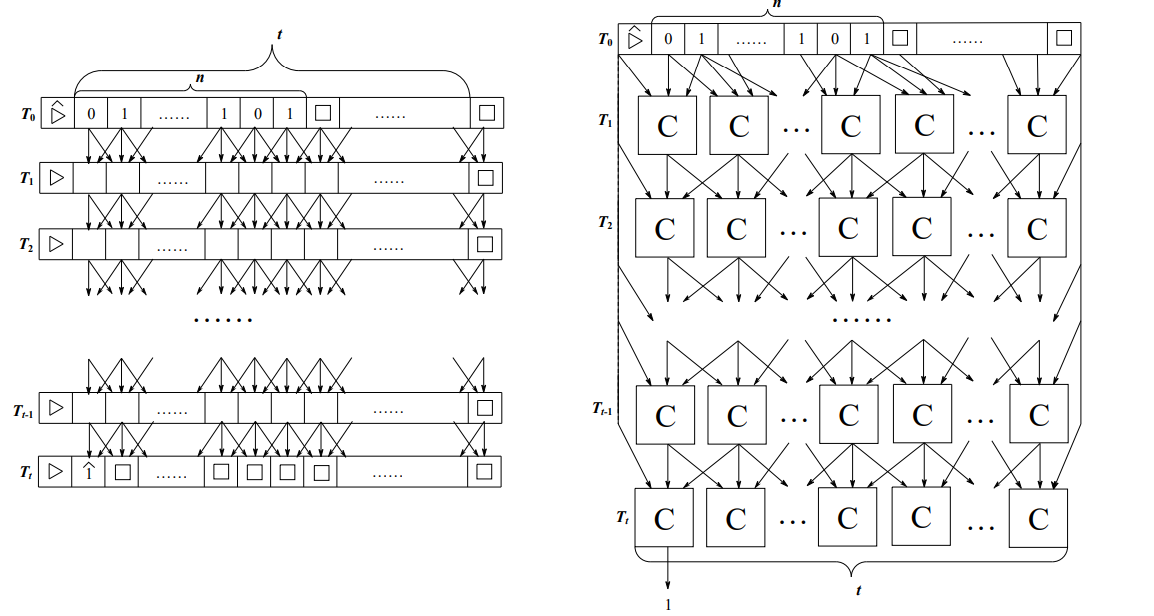
\includegraphics[width=5in]{fig.jpg}
		\caption{Reduction from TM to Circuit}
	\end{figure}
	$T_i$ are configurations. The symbols in $T_i$ only relies on at most 3 symbols in $T_{i-1}$. Therefore, the reduction can is computable in logspace.
	\item If a language has logspace-uniform circuits, then there is an implicitly logspace
	computable function mapping $1^n$ to $C_n$. Therefore the language is in P. 
\end{enumerate}
\end{solution}


\end{document}